\documentclass[aspectratio=169]{beamer}
\usepackage[utf8]{inputenc}
\usepackage{hyperref}
\usepackage{amsmath,amsfonts,amsthm,bm}
\usepackage{color}
\usepackage{minted}
\usepackage{graphicx} % Allows including images
\usepackage{booktabs} % Allows the use of \toprule, \midrule and \bottomrule in tables
\usepackage{tikz}
\usepackage[version=3]{mhchem}
\usepackage{pgfplots}
\pgfplotsset{compat=1.16} 
\setminted{fontsize=\scriptsize}
\newcommand{\classname}{NANOx81R}

\hypersetup{
    colorlinks=true,
    linkcolor=red,
    filecolor=magenta,      
    urlcolor=red,
}

\DeclareMathOperator*{\argmax}{argmax}
\DeclareMathOperator*{\argmin}{argmin}
\let \vec \mathbf

\mode<presentation> {
    \usetheme{CambridgeUS}
    \setbeamertemplate{footline}[text line]{%
      \parbox{\linewidth}{\vspace*{-8pt}\classname\hfill\insertpagenumber}}

    %\setbeamertemplate{footline}[page number]
    \setbeamertemplate{navigation symbols}{}
}


\title[Improving and Extending Linear Models]{Improving and Extending Linear Models}

\author{Shyue Ping Ong}
\institute[UCSD]{Aiiso Yufeng Li Family Department of Chemical and Nano Engineering\\
University of California, San Diego\\\url{http://materialsvirtuallab.org}}
\date{}

\begin{document}


\begin{frame}
    \titlepage % Print the title page as the first slide
\end{frame}


\begin{frame}{Overview}
    \tableofcontents
\end{frame}


\section{Preliminaries}

\begin{frame}{Preliminaries}
    \begin{itemize}
        \item In this lecture, we will look at various approaches to improving and extending simple linear models.
        \item It is important to note that techniques and concepts such as regularization, shrinkage and transformation of inputs are general and extend to other models.
    \end{itemize}
\end{frame}


\section{Improving on linear models}


\begin{frame}{Improving on linear models}
    \Huge{\centerline{Improving on linear models}}
\end{frame} 

\begin{frame}{Feature selection}
    \begin{itemize}
        \item Often, we want to improve on the least squares model.
        \begin{itemize}
            \item To improve prediction accuracy by sacrificing some bias for reduced variance.
            \item To improve interpretability by reducing number of features or descriptors.
        \end{itemize}
        \item Three main approaches:
        \begin{enumerate}
            \item Subset selection
            \item Shrinkage methods
            \item Dimension reduction
        \end{enumerate}
    \end{itemize}
\end{frame}


\subsection{Subset selection}

\begin{frame}{Subset selection}
    Best subset selection
    \begin{itemize}
        \item Brute force approach.
        \item From $p$ parameters, find the subset of $k$ parameters that results in the smallest RSS.
        \item Combinatorially expensive for large $p$ and large $k$.
        \item Note that the best subset for a larger $k$ does not necessarily include the best subset for a smaller $k$.
    \end{itemize}
    Forward- or backward-stepwise selection
    \begin{itemize}
        \item Forward: Start with intercept, and iteratively add feature that most improves the fit.
        \item Backward: Start with full model, and sequentially deletes the feature with least impact on the fit.
    \end{itemize}
\end{frame} 


\subsection{Shrinkage}

\begin{frame}{Shrinkage methods}
    \begin{itemize}
        \item Subset methods is discrete, i.e., retains/discards variables, and tends to exhibit high variance.
        \item Shrinkage methods are more continuous and do not suffer as much from high variability.
        \item Basic concept: instead of finding the parameters that minimizes the RSS only, we add a penalty term that penalizes more complex models, e.g., models with larger coefficients or larger number of coefficients. This ``shrinks'' the coefficients, in some cases, to 0.
    \end{itemize}
\end{frame}


\begin{frame}{Ridge regression ($L_2$ regularization)}
    \begin{equation*}
        \hat{\beta^{ridge}} = \argmin_\beta \left \{ \sum_{i=1}^N (y_i - \beta_0 - \sum_{j=1}^p \beta_j x_j)^2 + \lambda \sum_{j=1}^p \beta_j^2 \right \}
    \end{equation*}
    \begin{itemize}
        \item $\lambda \geq 0$ is the shrinkage parameter. The larger the $\lambda$, the greater the shrinkage.
        \item Also equivalent to:
        \begin{eqnarray*}
        \hat{\beta^{ridge}} = \argmin_\beta \sum_{i=1}^N (y_i - \beta_0 - \sum_{j=1}^p \beta_j x_j)^2\\
        \mathrm{subject~to} \sum_{j=1}^p \beta_j^2 \leq t
        \end{eqnarray*}
    \end{itemize}
\end{frame}


\begin{frame}{Ridge regression - Key details}
    \begin{itemize}
        \item Intercept ($\beta_0$) is not part of penalty term.
        \item Inputs should be scaled prior to performing ridge regression, typically by centering to the mean and scaling to unit variance:
        \begin{equation*}
            z_j = \frac{x_j - \mu_{x_j}}{s_{x_j}}
        \end{equation*}
    \end{itemize}
\end{frame} 


\begin{frame}{LASSO ($L_1$ regularization)}
    \begin{equation*}
        \hat{\beta^{LASSO}} = \argmin_\beta \left \{ \sum_{i=1}^N (y_i - \beta_0 - \sum_{j=1}^p \beta_j x_j)^2 + \lambda \sum_{j=1}^p |\beta_j| \right \}
    \end{equation*}
    \begin{itemize}
        \item Least Absolute Shrinkage and Selection Operator
        \item $\lambda \geq 0$ is the shrinkage parameter. The larger the $\lambda$, the greater the shrinkage.
        \item Also equivalent to:
        \begin{eqnarray*}
        \hat{\beta^{LASSO}} = \argmin_\beta \sum_{i=1}^N (y_i - \beta_0 - \sum_{j=1}^p \beta_j x_j)^2\\
        \mathrm{subject~to} \sum_{j=1}^p |\beta_j| \leq t
        \end{eqnarray*}
    \end{itemize}
\end{frame}


\begin{frame}{LASSO regression - Key details}
    \begin{itemize}
        \item Intercept ($\beta_0$) is not part of penalty term.
        \item Inputs should be scaled prior to performing lasso regression, just as in ridge regression.
    \end{itemize}
\end{frame} 


\begin{frame}{Subset vs ridge vs LASSO}
    \begin{itemize}
        \item Consider a set of orthonormal features.
        \begin{itemize}
            \item Ridge: proportional shrinkage. No coefficients are set to zero.
            \item LASSO: ``soft'' thresholding. Translates coefficients by a factor, truncating at zero.
            \item Best-subset: ``hard'' thresholding. Drops all coefficients below a certain threshold.
        \end{itemize}
    \end{itemize}
    \begin{figure}
    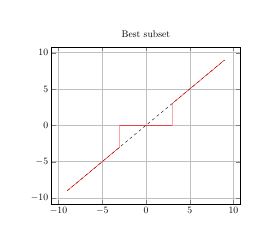
\begin{tikzpicture}[scale=0.35]
	\begin{axis}[title=Best subset, grid=major]
	\addplot[color=black, dashed] coordinates {
		(-9,-9)
		(9,9)
	};
	\addplot[color=red] coordinates {
		(-9,-9)
		(-3,-3)
		(-3,0)
		(3,0)
		(3,3)
		(9,9)
	};
	\end{axis}
	\end{tikzpicture}
    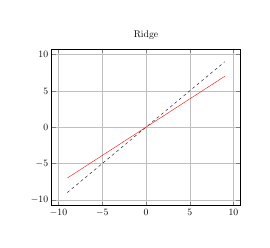
\begin{tikzpicture}[scale=0.35]
	\begin{axis}[title=Ridge, grid=major]
	\addplot[color=black, dashed] coordinates {
		(-9,-9)
		(9,9)
	};
	\addplot[color=red] coordinates {
		(-9,-7)
		(9,7)
	};
	\end{axis}
    \end{tikzpicture}
    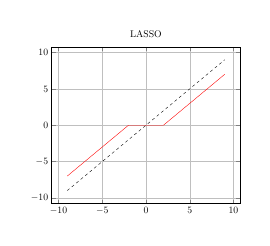
\begin{tikzpicture}[scale=0.35]
	\begin{axis}[title=LASSO, grid=major]
	\addplot[color=black, dashed] coordinates {
		(-9,-9)
		(9,9)
	};
	\addplot[color=red] coordinates {
		(-9,-7)
		(-2,0)
		(2,0)
		(9,7)
	};
	\end{axis}
    \end{tikzpicture}
        \includegraphics[width=0.35\textwidth]{figures/fig3-14.pdf}
    \end{figure}
\end{frame} 


\begin{frame}{Other variants of shrinkage methods}
    \begin{itemize}
        \item Elastic net penalty:
        \begin{eqnarray*}
            \lambda \left( \alpha \sum_{j=1}^p \beta_j^2+ (1-\alpha) \sum_{j=1}^p |\beta_j| \right)
        \end{eqnarray*}
        \item Least angle regression
    \end{itemize}
\end{frame}


\subsection{Derived input directions}

\begin{frame}{Derived input directions}
    \begin{itemize}
        \item General concept: transforms input $\vec{X}$ into a smaller subset of $\vec{z_m}$ and regress on $\vec{z_m}$
        \item Principal component regression:
        \begin{itemize}
            \item Transform non-orthonormal features into orthonormal directions using Principal Component Analysis (PCA).
            \item Choose $M$ directions that have the highest eigenvalues (explains the most variance) and discards the rest.
            \item Will revisit at a later lecture.
        \end{itemize}
    \end{itemize}
\end{frame} 


\begin{frame}{Partial Least Squares (PLS)}
    \begin{itemize}
        \item Algorithm:
        \begin{enumerate}
            \item Compute $\phi_{1j} = <\vec{x_j}, \vec{y}>$ for each $j$.
            \item First transformed direction $\vec{z_1} = \sum_j \phi_{1j} \vec{x_j}$, i.e., each direction is weighted by strength of effect on $\vec{y}$.
            \item Regress $\vec{y}$ on $\vec{z_1}$ to obtain $\theta_1$, orthogonalize $\vec{x_1}, ... \vec{x_p}$ wrt $\vec{z_1}$ via $x_j' = x_j - \frac{<\vec{z_1}, \vec{x_j}>}{<\vec{z_1}, \vec{z_1}>}\vec{z_1}$.
            \item Repeat until $M \leq p$ coefficients are obtained.
        \end{enumerate}
        \item Finds directions with high variance and high correlation with response.
    \end{itemize}
\end{frame} 


\section{Extending linear methods}

\begin{frame}{Preliminaries}
    \begin{itemize}
        \item It is highly unlikely that the true function $f(X)$ is linear in $X$.
        \item In some cases, linearity is a reasonable assumption, e.g., a first order Taylor series expansion:
        \begin{equation*}
            f(x) = f(a) + f'(a) (x-a) + f''(a) \frac{(x-a)^2}{2!} + f'''(a) \frac{(x-a)^3}{3!} + ...
        \end{equation*}
        \item Examples where this is used in materials science - linear elasticity (Hooke's law), etc.
        \item More frequently, we perform a transformation of inputs to create a linear basis expansion.
    \end{itemize}
\end{frame}


\section{Transformation of inputs}

\begin{frame}{General concept}
    \begin{itemize}
        \item Express:
        \begin{equation*}
            f(X) = \sum_{m=1}^M \beta_m h_m(X)
        \end{equation*}
        where $h_m$ is the $m^{th}$ transformation of $X$.
        \item This is known as a linear basis expansion in $X$.
        \item The key lies in choice of the basis functions $h_m$.
    \end{itemize}
\end{frame}

\begin{frame}{Examples of basis expansions}
    \begin{itemize}
        \item $h_m(X) = X_j^2, h_m(X) = X_i X_j$
        \begin{itemize}
            \item Polynomial expansion to higher-order Taylor series terms.
            \item No. of terms increases exponentially with degree of polynomial. For $p$ variables, we have $O(p^2)$ square and cross-product terms in a quadratic model. For a degree $d$ polynomial, we have $O(p^d)$.
        \end{itemize}
        \item $h_m(X) = log(X_j), sqrt(X_j), exp(i X_j)$: non-linear transformations in $X$.
        \item $h_m(X) = I(L_m \leq X_k < U_m)$: Piece-wise division of regions of $X$. E.g., cubic splines.
        \item $h_m(X) = RBF(||X-X_m||)$: radial basis function, e.g., Gaussian. 
        \item Typically, basis functions are used simply to allow a more flexible representation of the data. The basis functions can span a very large (sometimes infinite) set, from which a selection has to be made:
        \begin{itemize}
            \item Restriction - Truncate the choice of basis functions using some criteria.
            \item Selection - Choose basis functions that contribute significantly to the fit.
            \item Regularization - Use the whole and/or very large subset and apply regularization techniques (e.g., ridge or LASSO) to restrict coefficients.
        \end{itemize}
    \end{itemize}
\end{frame}

\begin{frame}{Linearization from physical laws}
    \begin{itemize}
        \item Arrhenius law:
        \begin{equation*}
            r = A \exp(-\frac{E_a}{RT}) \longrightarrow log(r) = log(A) - \frac{E_a}{RT}
        \end{equation*}
        \item Ising model:
        \begin{equation*}
            H(\sigma) = - \sum_{<i, j>} J_{ij}\sigma_i \sigma_j - \mu \sum_j h_j \sigma_j
        \end{equation*}
        \begin{figure}
            \centering
            \includegraphics[width=0.3\textwidth]{figures/ising.png}
        \end{figure}
    \end{itemize}
\end{frame}


\begin{frame}{Compressive sensing for cluster expansions}
    \begin{itemize}
        \item Cluster expansion of energy on lattice points:
        \begin{equation*}
            H(\sigma) = E_0 + \sum_f J_f \prod_f(\sigma)
        \end{equation*}
        \item $\sigma$ is the vector representing occupation of lattice sites, $\prod_f$ are the cluster basis functions, $J_f$ are effective cluster interactions (ECIs).
        \item Compressive sensing: essentially a LASSO to solve for ECIs.\cite{nelsonCompressiveSensingParadigm2013}
        \begin{figure}
            \centering
            \includegraphics[width=0.3\textwidth]{figures/numberofclusters.png}
            \includegraphics[width=0.3\textwidth]{figures/ecifit.pdf}
        \end{figure}
    \end{itemize}
\end{frame} 

\section{Piece-wise polynomials}

\begin{frame}{Piecewise polynomials}
    \begin{equation*}
        h_1(X) = I(X < \xi_1), h_2(X) = I(\xi_1 \leq X < \xi_2), h_3(X) = I(X \geq \xi_2)
    \end{equation*}
    \begin{columns}
    \column{0.3\textwidth}
    \begin{figure}
        \centering
        \includegraphics[width=\textwidth]{figures/piecewisefits.pdf}
    \end{figure}
    \column{0.7\textwidth}
    Parameters:
    \begin{itemize}
        \item No. of knots
        \item Order of polynomial
        \item Continuity at knots (value, first derivative, second derivative, etc.). For a polynomial of order $N$, we usually want all derivatives $< N$ to be continuous. 
    \end{itemize}
    \end{columns}
\end{frame} 


\begin{frame}{Cubic splines}
    \begin{columns}
    \column{0.5\textwidth}
    \begin{figure}
        \centering
        \includegraphics[width=0.7\textwidth]{figures/piecewisecubic.pdf}
    \end{figure}
    \column{0.5\textwidth}
    \begin{itemize}
        \item Probably the most commonly used.
        \item Continuous 1st and 2nd derivatives.
        \item Natural cubic spline: polynomial is linear beyond boundaries.
        \item Smoothing spline: Use  regularization to control complexity:
        \begin{eqnarray*}
            RSS(f, \lambda) = \sum_{i=1}^N \{y_i - f(x_i)\} ^ 2 \\
            + \lambda \int \{f''(t)\}^2 dt
        \end{eqnarray*}
    \end{itemize}
    \end{columns}
\end{frame}


\begin{frame}{Examples of cubic spline fitting}
    \begin{itemize}
        \item Spline-based Modified Embedded Atom Method (MEAM)
        \begin{eqnarray*}
            E = \sum_{i <j} \phi(r_{ij}) + \sum_i U(n_i), \\
            n_i = \sum_j \rho(r_{ij}) + \sum_{i < k, j,k!=i} f(r_{ij}) f(r_{ik})g[cos(\theta_{jik})]
        \end{eqnarray*}
        where $\phi$, $U$, $\rho$, $f$ and $g$ can be approximated by cubic splines. 
        \begin{figure}
            \centering
            \includegraphics[width=0.3\textwidth]{figures/meam-phi.png}
            \includegraphics[width=0.3\textwidth]{figures/meam-u.png}

        \end{figure}
    \end{itemize}
\end{frame} 


\begin{frame}[fragile]{Demo: Cubic spline fitting in scipy}
    \inputminted{python}{example_sklearn_spline.py}
\end{frame} 


\section{Gaussian basis functions}


\begin{frame}{Gaussian basis functions}
    \begin{equation*}
        h_m(x) = \exp(-k(x - x_m) ^ 2)
    \end{equation*}
    \begin{itemize}
        \item Gaussian functions centered at $x_m$.
        \item Other similar types of functions include Lorentzian ($h_m(x) = \frac{1}{1 + kx^2}$), Gaussian-Lorentzian, Voigtian, Pearson type IV, and beta profiles.
    \end{itemize}
\end{frame} 


\begin{frame}{Example: Rietveld refinement}
\begin{figure}
    \centering
    \includegraphics[width=0.45\textwidth]{figures/rietveld.pdf}
    \caption{Neutron powder diffraction diagram of \ce{CaUO4}}
\end{figure}
    \begin{itemize}
        \item Least squares fitting of theoretical line profile to match a measured diffraction pattern (e.g., X-ray, neutron).\cite{rietveldProfileRefinementMethod1969}
    \end{itemize}
\end{frame} 


\begin{frame}{Example: Rietveld refinement, contd.}
    \begin{itemize}
        \item Peak shape function:
        \begin{equation*}
            PSF(\theta) = \Omega(\theta) \otimes \Lambda(\theta) \otimes \Psi(\theta) + b(\theta)
        \end{equation*}
        \item $\Omega$: Instrument broadening, $\Lambda$: Wavelength dispersion, $\Psi$: Specimen function.
        \item For single phase, minimize:
        \begin{equation*}
            \Phi = \sum_{i=1}^N w_i \left ( Y_i^{obs} - \left ( b_i + K \sum_{j=1}^m I_jy_j(x_j)\right )\right )^2
        \end{equation*}
        \item where $y_j(x_j)$ is typically a pseudo-Voigt (mix of Gaussian and Lorentizan function) function.
        \item Note that the background ($b_i$) holds no useful structural information and should be minimized in experiments.
    \end{itemize}
\end{frame} 



\section{Wavelet and Fourier basis functions}


\begin{frame}
\frametitle{Wavelet smoothing}
\begin{columns}
\column{0.4\textwidth}
\begin{figure}
    \centering
    \includegraphics[width=\textwidth]{figures/wavelets.pdf}
\end{figure}
\column{0.6\textwidth}
    \begin{itemize}
        \item Complete orthonormal basis
        \item Shrink and select toward \textbf{sparse} representation.
        \item Able to represent both time and frequency localization efficiently (Fourier basis can only do frequency localization).
    \end{itemize}
\end{columns}
\end{frame} 


\begin{frame}{Example: NMR Spectroscopy}
\begin{columns}
\column{0.4\textwidth}
\begin{figure}
    \centering
    \includegraphics[width=0.45\textwidth]{figures/nmrwavelet.pdf}
    \caption{Subtraction of a large spectral line: (top) the original spectrum of polyethylene, (bottom) reconstructed spectrum after removal of \ce{CH2} peak.\cite{baracheContinuousWaveletTransform1997}}
\end{figure}
\column{0.6\textwidth}
    Applications:
    \begin{itemize}
        \item Suppression of large unwanted spectral line (left).
        \item Rephasing spectrum perturbed by time-dependent magnetic field.
        \item Noise filtering
        \item Detecting phases in a mixture
    \end{itemize}
\end{columns}
\end{frame} 

\begin{frame}{Example: Fourier transform for analysis of extended X-ray absorption fine structure (EXAFS)}
    
    \begin{columns}
    \column{0.2\textwidth}
    \begin{figure}
        \centering
    \includegraphics[width=\textwidth]{figures/EXAFS-1.png}
    \includegraphics[width=\textwidth]{figures/EXAFS-2.png}
    \includegraphics[width=\textwidth]{figures/EXAFS-3.png}
    \end{figure}
    \column{0.77\textwidth}
    \begin{itemize}
        \item (a) The extended edge (orange part) contains information of atom chemical environment.
        \item (b) Subtract the background, convert energy to k-space unit, and multiply the normalized intensity by $k^2$
        \item (c) Fourier transform $k$-space information to real space and obtain the first shell bond length. 
    \end{itemize}
    \end{columns}
\end{frame} 


\begin{frame}[allowframebreaks]{Bibliography}
    \bibliographystyle{unsrt}
    \bibliography{refs}
\end{frame}


\begin{frame}
    \Huge{\centerline{The End}}
\end{frame}

\end{document}

